% EPC flow charts
% Author: Fabian Schuh
\documentclass{article}
\usepackage[inner=0.5in,outer=0.5in,top=0.25in,bottom=0.25in]{geometry}
\usepackage{xeCJK} % 分開設置中英文字型
\setCJKmainfont{微軟正黑體} % 設定中文字型
\usepackage{enumitem}
\usepackage{graphicx}
\usepackage{tikz}
\usetikzlibrary{positioning,arrows}
\usetikzlibrary{shapes.multipart}

\tikzset{
    state/.style={
           rectangle,
           rounded corners,
           draw=black,
           minimum height=2em,
           inner sep=2pt,
           text centered,
           },
}
\tikzset{
    phantom/.style={
           rectangle,
           rounded corners,
           minimum height=2em,
           inner sep=2pt,
           text centered,
           },
}
\setlist[enumerate]{topsep = 0pt, noitemsep}%remove extra empty spaces above enumerate envr, and make the items more compact

\begin{document}
\tikzstyle{abstract}=[rectangle, draw=black, rounded corners,  anchor=center, text width=3cm,text centered,rectangle split, rectangle split parts=2]

\begin{tikzpicture}[item/.style={draw=black, rounded corners,  anchor=center, text width=8.5cm,align = center,rectangle split, rectangle split parts=#1, rectangle split part align={center, left} }]

\begin{scope}[node distance=5mm and 5mm]

\node [ item=2](a) at (1,1) {%
            \textbf{未完成方向}
            \nodepart{two}
            \begin{enumerate}
            	\item share community, tikz, LYX doc, ...
            	\item Math.lyx與.pdf清楚化
            	\item LYX做webpost時的標題列css模組化
            	\item 軟體學習、紀錄、分享。
            	\item 軟體升級成texlive 2017?
            	\item sciencefair typeset conti, 將疊格繪圖方程modulize.
           \end{enumerate}
            };

\node [phantom, inner sep = 0pt, right=of a.north east](center_point){};

\node [above = of center_point, align = center] (title){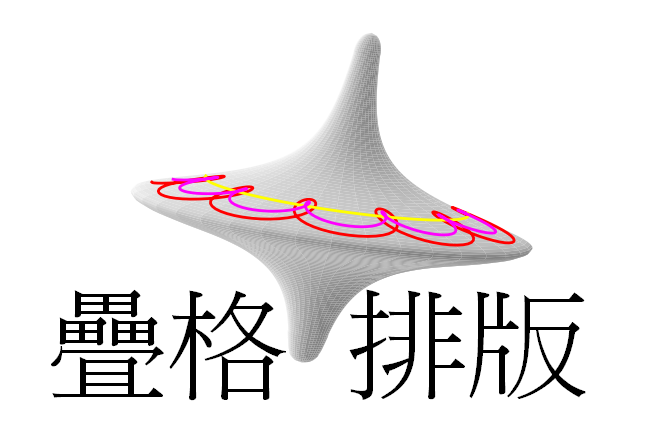
\includegraphics[width=0.4\textwidth]{../../figs/tex_logo.png}\\ \LARGE 事業部規劃};

\node [state,below=of a](b)
{git log}edge [<-,>=stealth'] (a);

\node [ item=2, right = of center_point, anchor = north west](unique) {%
            \textbf{特色}
            \nodepart{two}
            \begin{enumerate}
            	\item 使用LYX與SW,高度自動化(省下很多細微瑣碎步驟)。
            	\item 與不同應用做方便性整合,如django,web blog等等。
           \end{enumerate}
            };

\node [ item=2,below = of b](small) {%
            \textbf{未完成細項}
            \nodepart{two}
            \begin{enumerate}
            	\item 總經排
            	\item chemgreek目前是放在同目錄下,需裝成package。
            	\item LYX export包含有被伺服圖檔的html檔,目前已有一寫下的流程,但還是要做成自動化較方便。
            	\item vec A不對稱問題,A*正確的方式?
            	\item 順著陀螺外型的powered by LYX SW字串,path?
            	\item 加入tikz說明書,node position,anchor參數必須要在above right之類參數之後才會有效。
           \end{enumerate}
            };

\end{scope}
\end{tikzpicture}
\end{document}